\documentclass{nithreport}

\usepackage{graphicx}

\title{Program Dependence Maze}
\author{Pranav Kant}
\report{A major project}
\nithdegree{Bachelor of Technology}
\degreeshort{B.Tech.}
\reportmonth{May}
\reportyear{2015}
\projectstartdate{August, 2014}
\projectenddate{May, 2015}
\mentor{Kumar Sambhav Pandey}
\mentordesignation{Associate Professor}
\mentoraffiliation{Department of Computer Science and Engineering, National Institute of Technology Hamirpur}

\authors{{Pranav Kant (11512), Pranav Kant (11512),Pranav Kant (11512)}}

\begin{document}
  
\maketitle
\pagenumbering{roman}
\certificate


\begin{acknowledgments}
We take this opportunity to express our deepest gratitude and appreciation to all those who have helped us directly or indirectly towards the successful completion of this project.\\
First and foremost, we would like to express our sincere appreciation and gratitude. First and foremost, we would like to express our sincere appreciation and gratitude First and foremost, we would like to express our sincere appreciation and gratitude First and foremost, we would like to express our sincere appreciation and gratitude First and foremost, we would like to express our sincere appreciation and gratitude First and foremost, we would like to express our sincere appreciation and gratitude First and foremost, we would like to express our sincere appreciation and gratitude First and foremost, we would like to express our sincere appreciation and gratitude First and foremost, we would like to express our sincere appreciation and gratitude First and foremost, we would like to express our sincere appreciation and gratitude First and foremost, we would like to express our sincere appreciation and gratitude First and foremost, we would like to express our sincere appreciation and gratitude First and foremost, we would like to express our sincere appreciation and gratitude First an and foremost, we would like to express our sincere appreciation and gratitude. First and foremost, we would like

to express our sincere appreciation and gratitude First and foremost, we would like to express our sincere appreciation and gratitude First and foremost, we would like to express our sincere appreciation and gratitude First and foremost, we would like to express our sincere appreciation and gratitude First and foremost, we would like to express our sincere appreciation and gratitude First and foremost, we would like to express our sincere appreciation and gratitude First and foremost, we would like to express our sincere appreciation and gratitude First and foremost, we would like to express our sincere appreciation and gratitude First and foremost, we would like to express our sincere appreciation and gratitude First and foremost, we would like to express our sincere appreciation and gratitude First and foremost, we would like to express our sincere appreciation and gratitude First and foremost, we would like to express our sincere appreciation and gratitude First an

\end{acknowledgments}

\tableofcontents
\listoftables
\listoffigures

\begin{abstract}
This is great abstract. This is great abstract.This is great abstract.This is great abstract.This is great abstract.This is great abstract.This is great abstract.This is great abstract.This is great abstract.This is great abstract.This is great abstract.This is great abstract.This is great abstract.This is great abstract.This is great abstract.This is great abstract.This is great abstract.This is great abstract.This is great abstract.This is great abstract.This is great abstract.This is great abstract.This is great abstract.This is great abstract.This is great abstract.This is great abstract.This is great abstract.This is great abstract.This is great abstract.This is great abstract.This is great abstract.This is great abstract.This is great abstract.This is great abstract.This is great abstract.This is great abstract.This is great abstract.This is great abstract.This is great abstract.This is great abstract.This is great abstract.This is great abstract.This is great abstract.This is great abstract.This is great abstract.This is great abstract.This is great abstract.This is great abstract.This is great abstract.This is great abstract.This is great abstract.This is great abstract.This is great abstract.This is great abstract.This is great abstract.This is great abstract.This is great abstract.This is great abstract.This is great abstract.
\end{abstract}

\pagenumbering{arabic}

\chapter{Introduction}
To bold any entry, you can {\bf do this}. To italicize, {\it do this}. For underline, you can \underline{use this}.

You can cite any entry in the corresponding .bib file. The corresponding .bib file for this sample.tex is refs.bib as mentioned by bibliography command at the bottom of document. The example refs.bib file only contains two entries as of now namely `small', `big'. You can use these to cite anything like this.\cite{big}. Citing the small one now like this\cite{small}. See the next paragraph to avoid indentation.

\noindent If you don't want to indent, start the paragraph like this (see latex code).

This is the introduction of the chapter. This is the introduction of the chapter. This is the introduction of the chapter. This is the introduction of the chapter. This is the introduction of the chapter. This is the introduction of the chapter. This is the introduction of the chapter.\cite{big} This is the introduction of the chapter. This is the introduction of the chapter. This is the introduction of the chapter. This is the introduction of the chapter. This is the introduction of the chapter. This is the introduction of the chapter. This is the introduction of the chapter. This is the introduction of the chapter. This is the introduction of the chapter. This is the introduction of the chapter. This is the introduction of the chapter. This is the introduction of the chapter. This is the introduction of the chapter. This is the introduction of the chapter. This is the introduction of the chapter. This is the introduction of the chapter. This is the introduction of the chapter. This is the introduction of the chapter. This is the introduction of the chapter. This is the introduction of the chapter.

\begin{figure}
  \centering % This keeps image horizontally centered.
  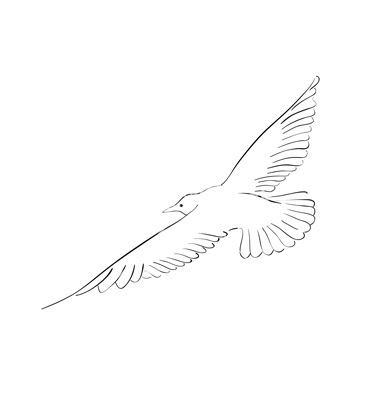
\includegraphics[width=2.5in, keepaspectratio]{gull.jpg}
  \caption{A picture of a gull}
\end{figure}

\begin{table}[h!]
\begin{tabular}{ | p{4in} | p{2in}| } 
 \hline
 {\bf Question} & {\bf Options} \\ 
 Hi, what's your name? & {\it Text field} \\ 
 What's your branch? & Computer Science, Electronics, Electrical \\
 Your year of engineering & First, second, third, final \\
 \hline
\end{tabular}
\caption{Table containing questions and options}
\end{table}

\section{Background}
THis adsf asdf

\subsection{PDG}
This is subsection of above section named Background.

\chapter{Motivation}
This is the motivation of the chapter. This is the motivation of the chapter. This is the motivation of the chapter. This is the motivation of the chapter. This is the motivation of the chapter. This is the motivation of the chapter. This is the motivation of the chapter. This is the motivation of the chapter. This is the motivation of the chapter. This is the motivation of the chapter. This is the motivation of the chapter. This is the motivation of the chapter. This is the motivation of the chapter. This is the motivation of the chapter. This is the motivation of the chapter. This is the motivation of the chapter. This is the motivation of the chapter. This is the motivation of the chapter. This is the motivation of the chapter. This is the motivation of the chapter. This is the motivation of the chapter. This is the motivation of the chapter. This is the motivation of the chapter. This is the motivation of the chapter. This is the motivation of the chapter. This is the motivation of the chapter. This is the motivation of the chapter. This is the motivation of the chapter. 

\bibliographystyle{IEEEtran}
\bibliography{refs}

\end{document}
